\mainchapter{Results}{0.6}{But I am not so bold as to think that things cannot take place differently from the way I have specified.}{Anonymous} \label{chap:results}

%----------------------------------------%
% Results
%----------------------------------------%

This thesis revolves around the implementation of a new inner boundary condition into the \flash\ code. Accordingly, much of the work involved an iterative process of trials and errors, where the implementation was tested with various parametrisations, and the results were carefully analysed in order to improve or correct the code. Beginning with the 1D simulations of the z9.6 progenitor, we present the quantities we analysed, what was expected from the outcome of the simulations, and the solutions we have developed to improve the results. We then present the 2D simulations of the s12 progenitor, where we address the impact of different wind velocities on the evolution.

\section{1D simulations \& testing} \label{sec:results_1d}

The simplest way to begin is with a one-dimensional simulation. It is easy to learn and understand the essential features of CCSNe simulations from the profiles of a 1D simulation. In addition, it is relatively cheap to perform, and the implementation can more easily be tested. However, the neutrino-driven mechanism generally fails to produce explosions in spherical symmetry because it cannot capture the effects of non-spherically symmetric phenomena, such as turbulence and instabilities, that would otherwise help shock revival. The z9.6 progenitor is one of the few low-mass progenitors known to successfully explode in 1D.

\clearpage

\subsection{Composition \& features} \label{sec:results_features}

To familiarise ourselves with the structure and features of the simulation, we begin by looking at profiles of the progenitor star at moment of collapse. \Cref{fig:z96_composition} shows the shell structure at the centre of the star, where we can clearly identify the iron core, extending to \(1.1 \cdot 10^8\units{cm}\), as well as the composition interfaces between the silicon and carbon+oxygen layers (Si/C+O) at \(1.45 \cdot 10^8\units{cm}\), and between the carbon+oxygen and the helium layers (C+O/He) at \(6.7 \cdot 10^8\units{cm}\). The He/H composition interface, located at a radius of \(1.4 \cdot 10^{12}\units{cm}\), does not appear on \Cref{fig:z96_composition}.

\begin{figure}[ht!]
    \centering
    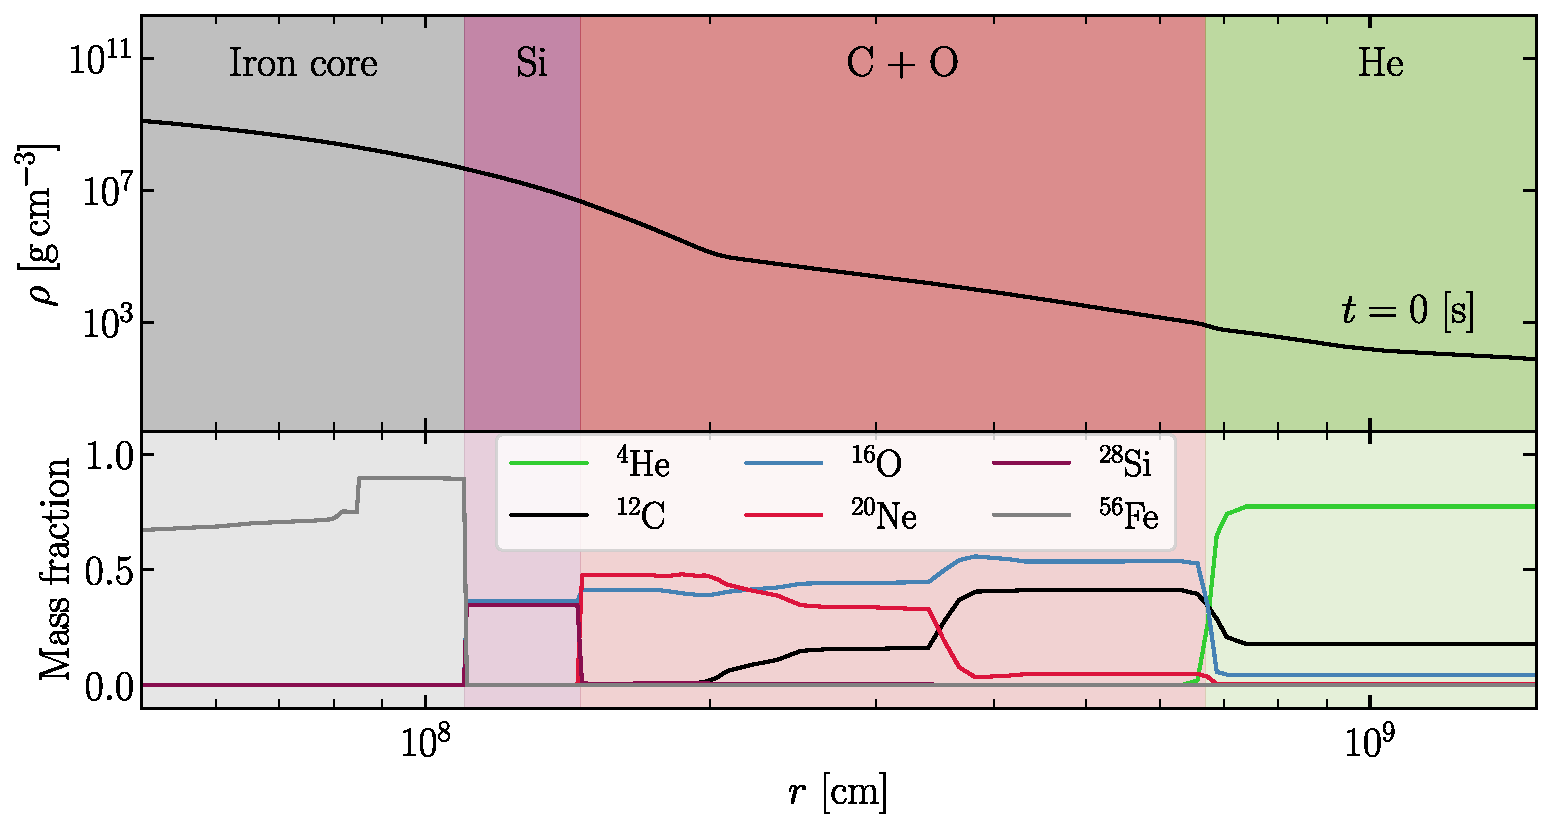
\includegraphics[width=1.0\linewidth]{figures/composition_1d.pdf}
    \caption{1D profile of the density \(\rho\) and the mass fractions of the main elements present in the depicted region, showing the core structure of the z9.6 progenitor at moment of collapse.}
    \label{fig:z96_composition}
\end{figure}

We then look at an evolved state of the simulation, at time of mapping \(t_\mathrm{map} = 1.6\units{s}\). At this point, the core has collapsed into a PNS, and the shock has propagated to a few thousand kilometres. \Cref{fig:z96_features} highlights the region of nuclear density corresponding to the location of the PNS, as well the \emph{forward shock} and the \emph{reverse shock}. The forward shock is the initial shock launched at time of bounce, which has been revived by neutrino heating and sweeps up the material in the outer layers of the star. The reverse shock propagates inward into the inner ejecta. As shown in \Cref{fig:z96_features}, the reverse shock is formed due to the ejecta being accelerated by the neutrino wind to supersonic speeds, and entering in contact with the shocked material behind the forward shock, causing a sharp drop in velocity and heating the material.

\begin{figure}[ht!]
    \centering
    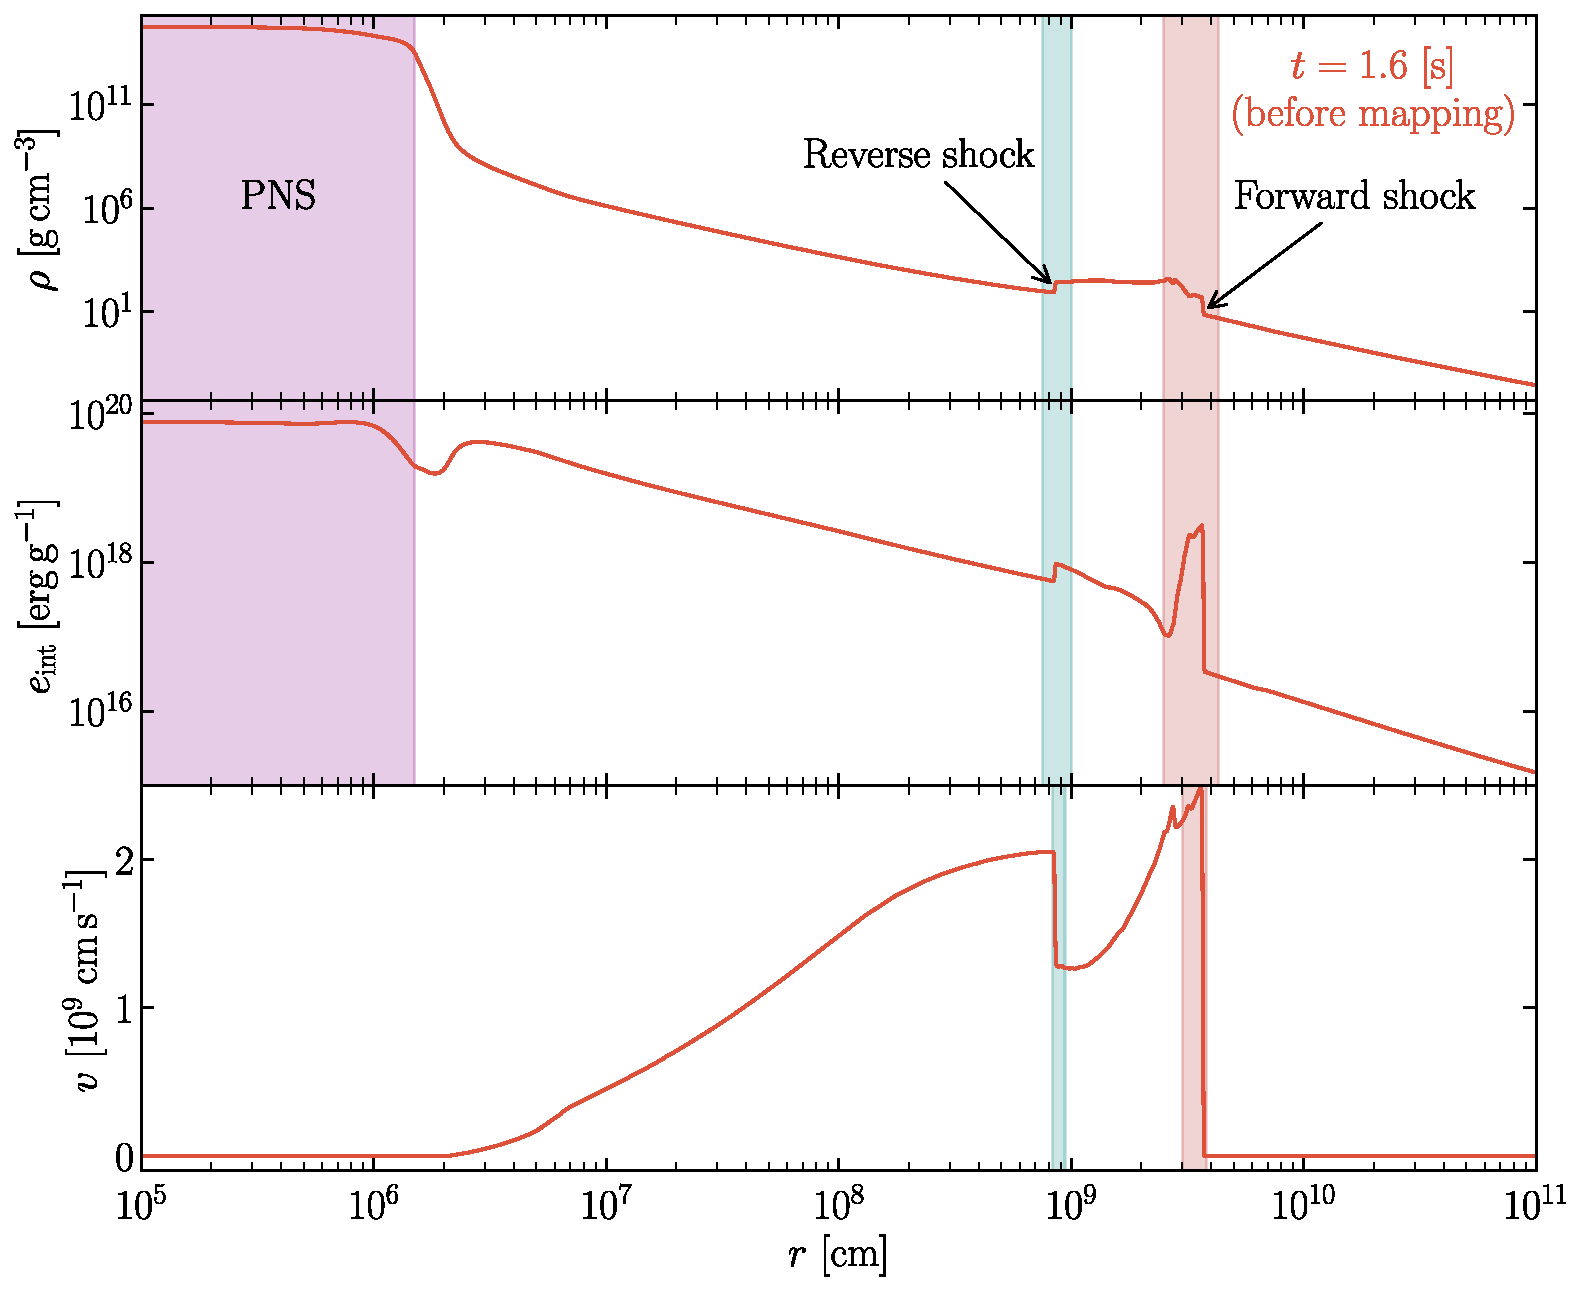
\includegraphics[width=1.0\linewidth]{figures/features_1d.pdf}
    \caption{1D profiles of the density \(\rho\), internal energy \(e_\mathrm{int}\), and velocity \(v\) for the initial simulation at time of mapping \(t_\mathrm{map} = 1.6\units{s}\) of the z9.6 progenitor. The region of nuclear density corresponding to the PNS is shown (purple region), as well as the discontinuities in thermodynamical state associated with the forward and reverse shocks (red and blue regions).}
    \label{fig:z96_features}
\end{figure}

\clearpage

\subsection{Spatial gradient} \label{sec:results_gradient}

The first implementation of the neutrino wind boundary condition prescribed constant values of density and internal energy inside the hole, following the model presented in \Cref{sec:bdry_out}. The velocity is kept constant at the inner boundary, but declines as \(\sqrt{r}\) inside the hole. This is done to prevent instabilities near \(r=0\), as the cells are still evolved in this region. Conveniently, this approximately matches the shape of the velocity profile from the initial 1D simulation near the inner boundary. The left panel of \Cref{fig:compare_grad} shows the result of a simulation ran until \(12\units{s}\) post-collapse with this first implementation. We see that the density profile outside the boundary matches the evolution of the initial simulation at \(1.6\units{s}\) and \(2.2\units{s}\). However, we note a rapid loss of velocity at the inner boundary that propagates to the reverse shock. This is not a desirable behaviour and could have a significant influence on the long-term evolution of the reverse shock. To attenuate this effect, we instead prescribe a spatial gradient profile to the density and internal energy inside the hole, that we express as power-laws in the same way as we did the time evolution presented in \Cref{sec:bdry_out}, but replacing the time variables with the radius. To find an adequate power-law index, we fit the density and internal energy profiles of the initial simulation in the same way as we fit the power-law index for the time evolution, again replacing the time variable with the radius. This would result in infinitely large density and internal energy near \(r=0\), defeating the purpose of the boundary condition. However, since we put the mass within the hole in a point mass, \flash\ does not compute the gravitational potential beyond a certain radius inside the hole, as this would result in a gravitational singularity at \(r=0\). This softening radius, \(r_\mathrm{soft}\), is set at \(250\units{km}\). To achieve approximate hydrostatic equilibrium, we only need to prescribe our spatial gradient between this radius and the inner boundary. The right panel of \Cref{fig:compare_grad} shows the results of this new implementation. We still note a discontinuity in the velocity profile at the inner boundary due to numerical issues, however, we see that the material at the reverse shock is still correctly accelerated and that the profile matches better with the initial simulation at \(2.2\units{s}\).

\begin{figure}[ht!]
    \centering
    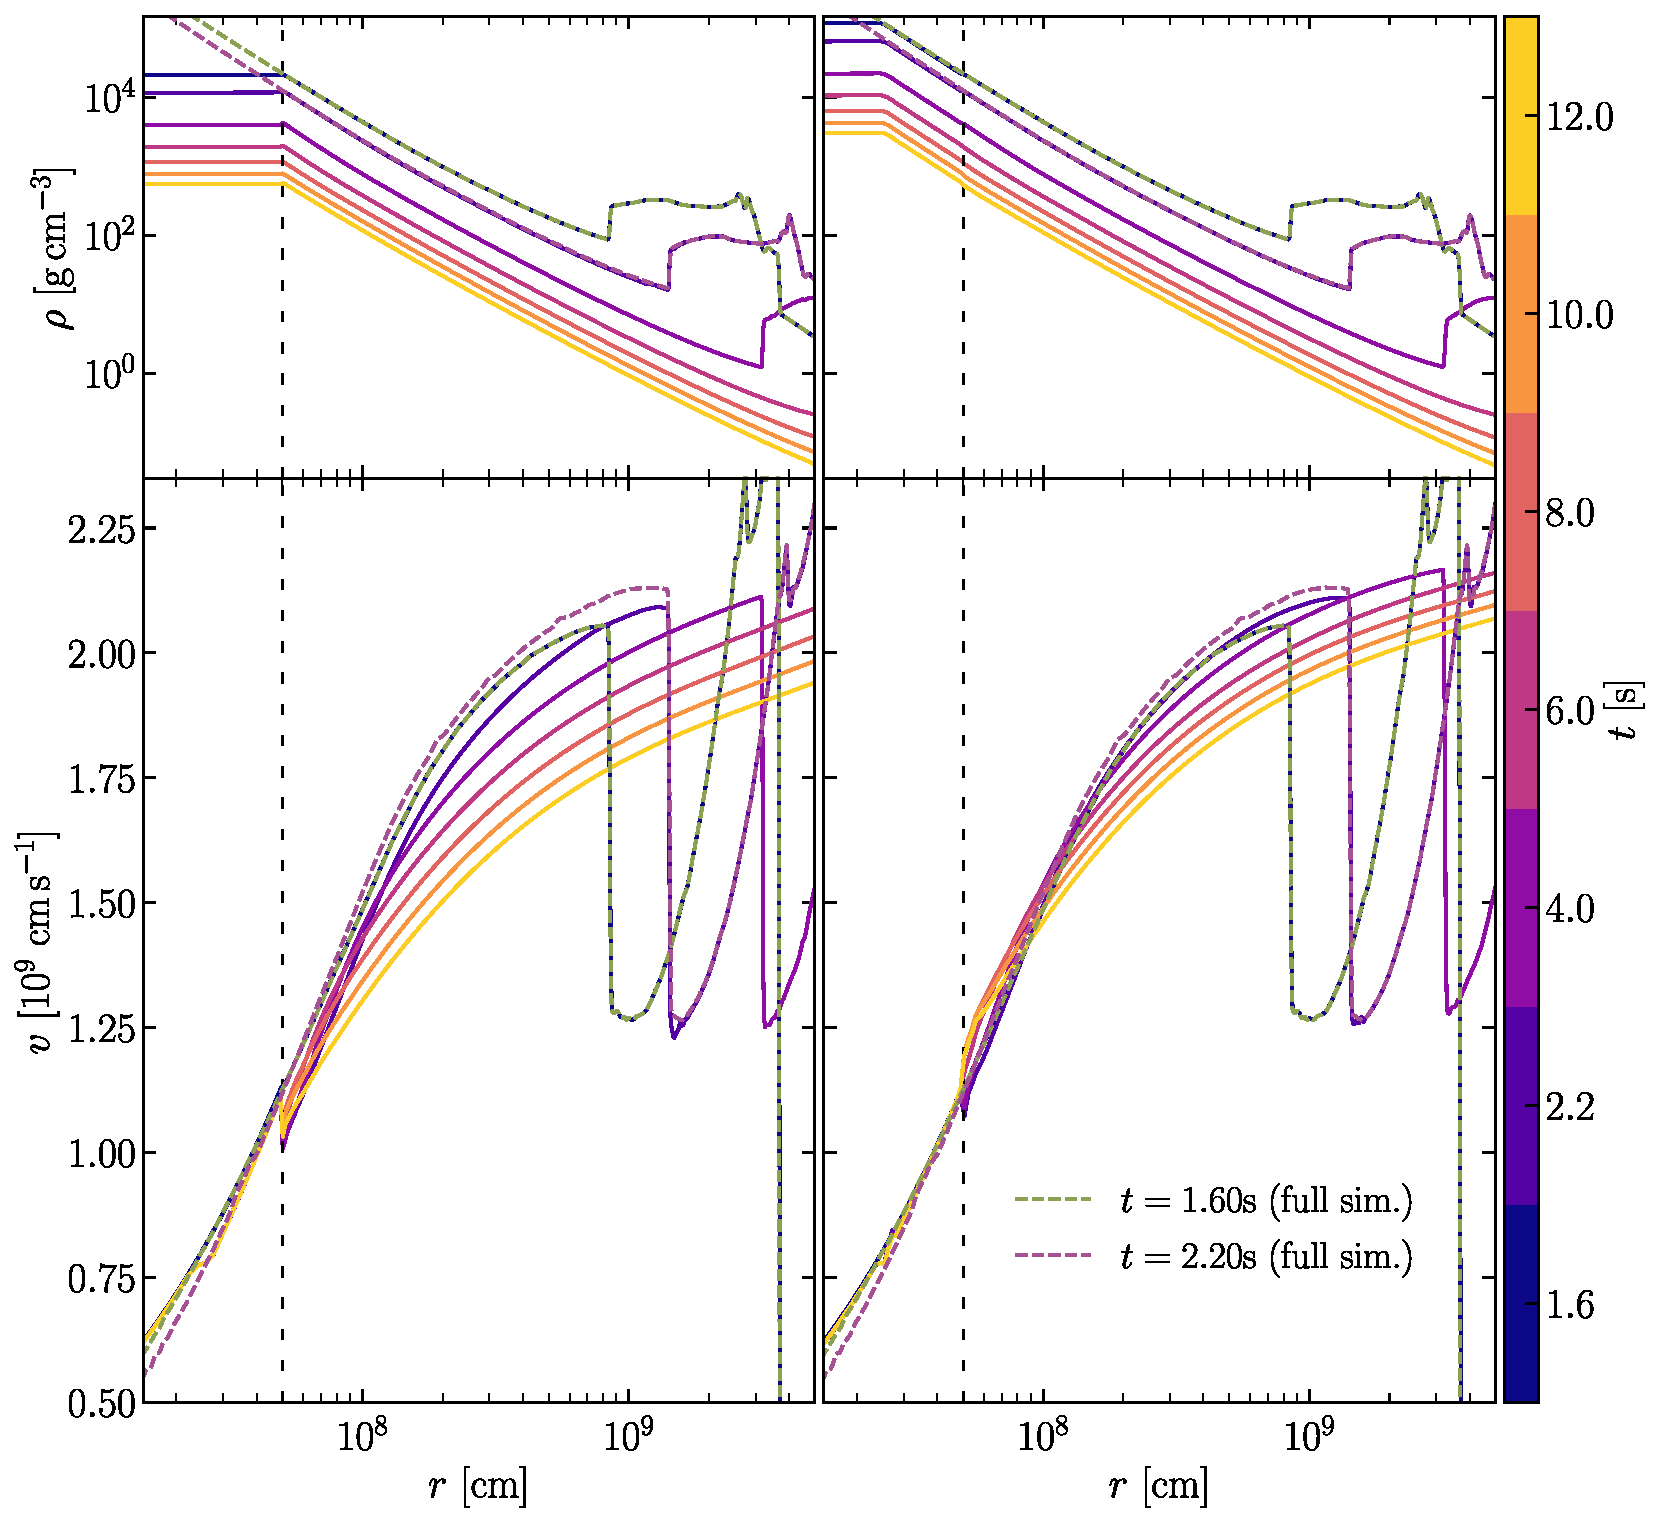
\includegraphics[width=1.0\linewidth]{figures/compare_grad.pdf}
    \caption{Comparison of the time evolution of the density and velocity near the inner boundary between a simulation without (left panel) and with approximate hydrostatic equilibrium inside the hole (right panel). The time evolution of the long term simulation (solid lines) is shown from time of mapping \(t_\mathrm{map} = 1.6\units{s}\) to \(12\units{s}\), and compared with profiles from the initial simulation (dashed lines) at \(1.6\units{s}\) and \(2.2\units{s}\).}
    \label{fig:compare_grad}
\end{figure}

\clearpage

\subsection{Long-term profiles}

We now look at the final results of the long-term simulation for the z9.6 progenitor. \Cref{fig:short_1d} shows a series of profiles of the density, internal energy and velocity from time of mapping to \(10\units{s}\) after collapse, on which we see the expansion of the forward shock, as well as the slower expansion of the reverse shock.

\begin{figure}[ht!]
    \centering
    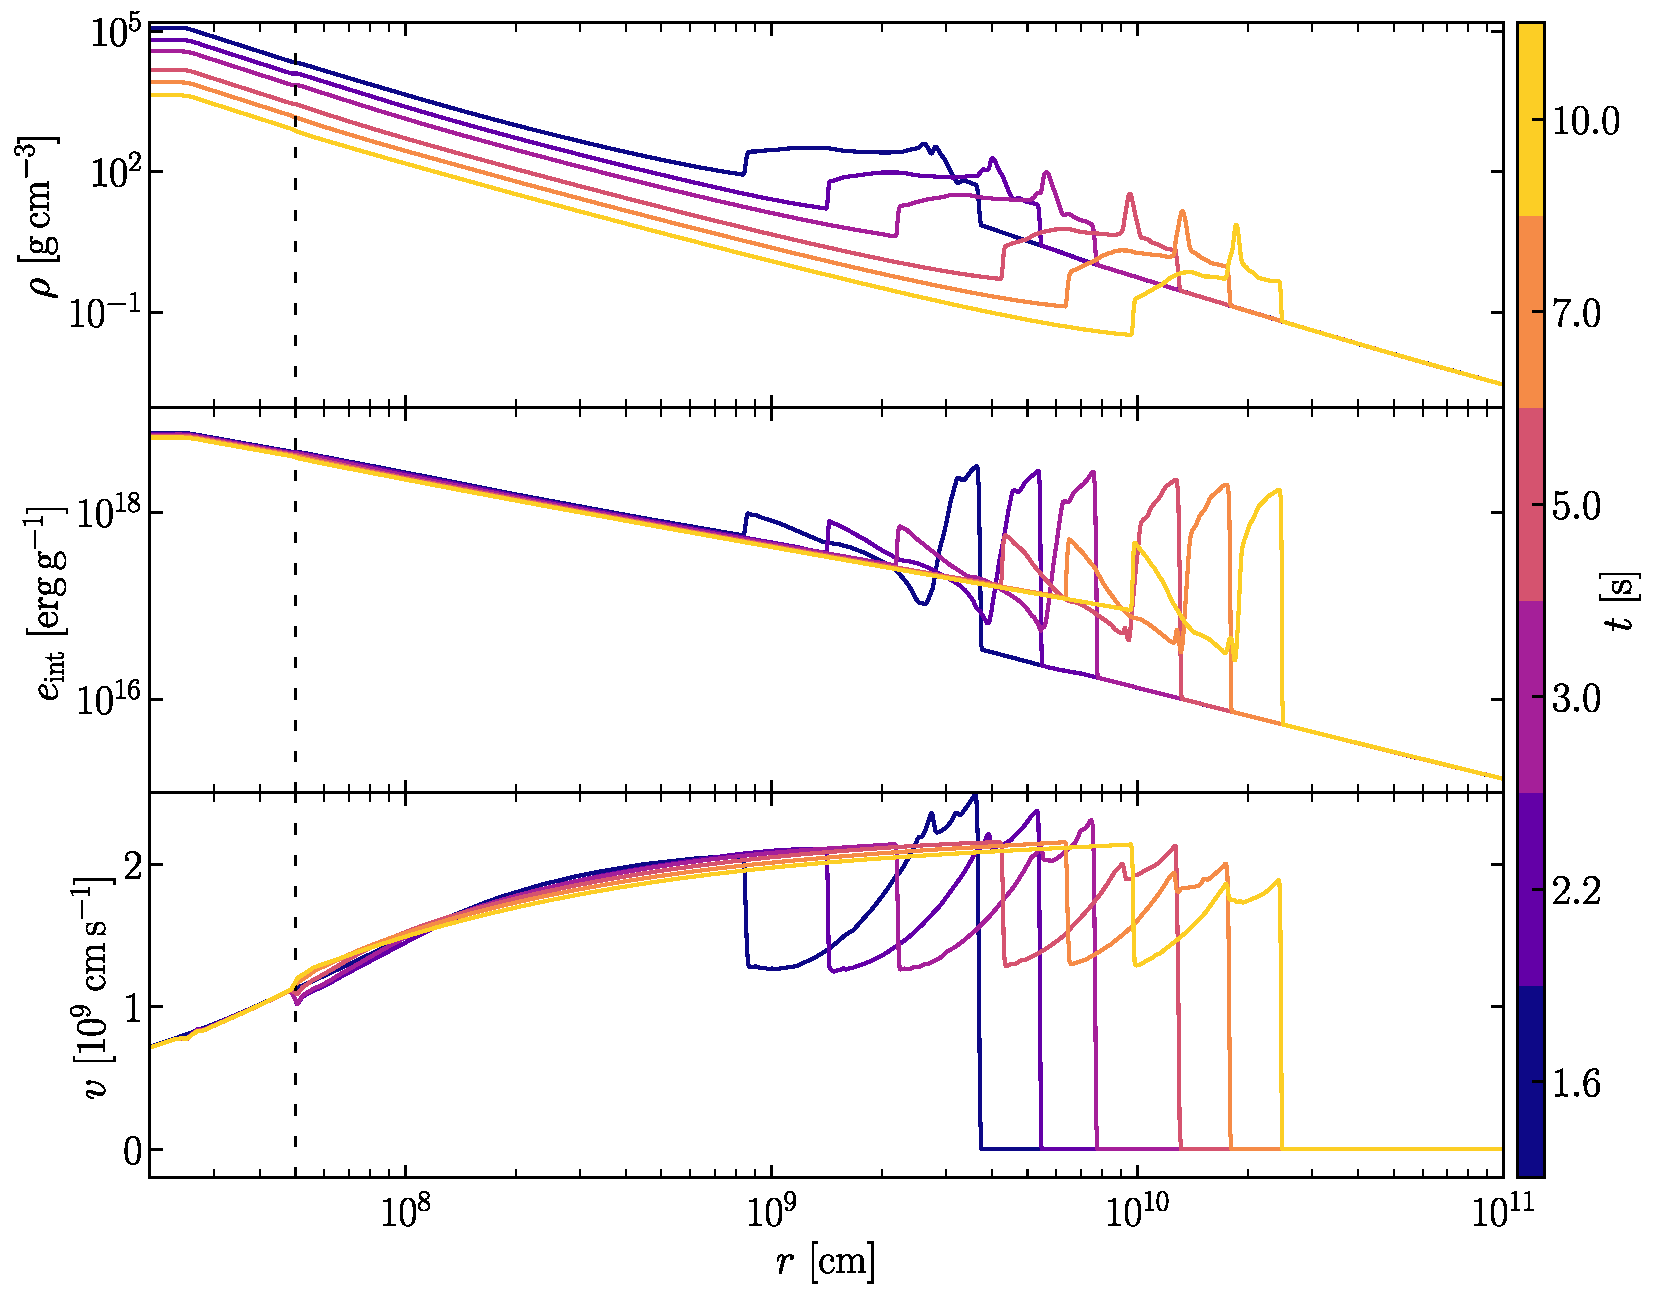
\includegraphics[width=1.0\linewidth]{figures/short_1d.pdf}
    \caption{1D profiles of the density \(\rho\), internal energy \(e_\mathrm{int}\) and velocity \(v\) from time of mapping \(t_\mathrm{map}\) to \(10\units{s}\) post-collapse. The neutrino wind boundary condition is used during this time, with the inner boundary located at \(r=500\units{km}\) (vertical black dashed line).}
    \label{fig:short_1d}
\end{figure}

\Cref{fig:long_1d} shows profiles of the evolution until shock breakout. At \(20\units{s}\), the density of the wind has already dropped to \(\sim10^2\units{g/cm^3}\). At \(30\units{s}\), the neutrino wind is replaced with the inflow boundary condition described in \Cref{sec:bdry_in}, in which the density and internal energy at the boundary are set to a fraction (1\%) of their values directly outside the boundary, producing a discontinuity at the boundary and a flat profile inside the hole. The velocity is also set to zero. At \(\sim100\units{s}\), the boundary has expanded to a radius of \(\sim8\cdot10^8\units{cm}\), and the reverse shock, at \(\sim8\cdot10^{10}\units{cm}\), begins to recede. We note that the behaviour of the reverse shock is influenced by the introduction of the inflow boundary condition, which shuts off the ejecta and causes a loss of pressure support in the centre, and may cause it to recede earlier than it otherwise would have. Much later, at \(\sim20{,}000\units{s}\), the boundary has expanded to its maximum radius of \(2\cdot10^{11}\units{cm}\), and after \(\sim100{,}000\units{s}\), the forward shock has reached the outer boundary of the domain, indicating shock breakout.

\begin{figure}[ht!]
    \centering
    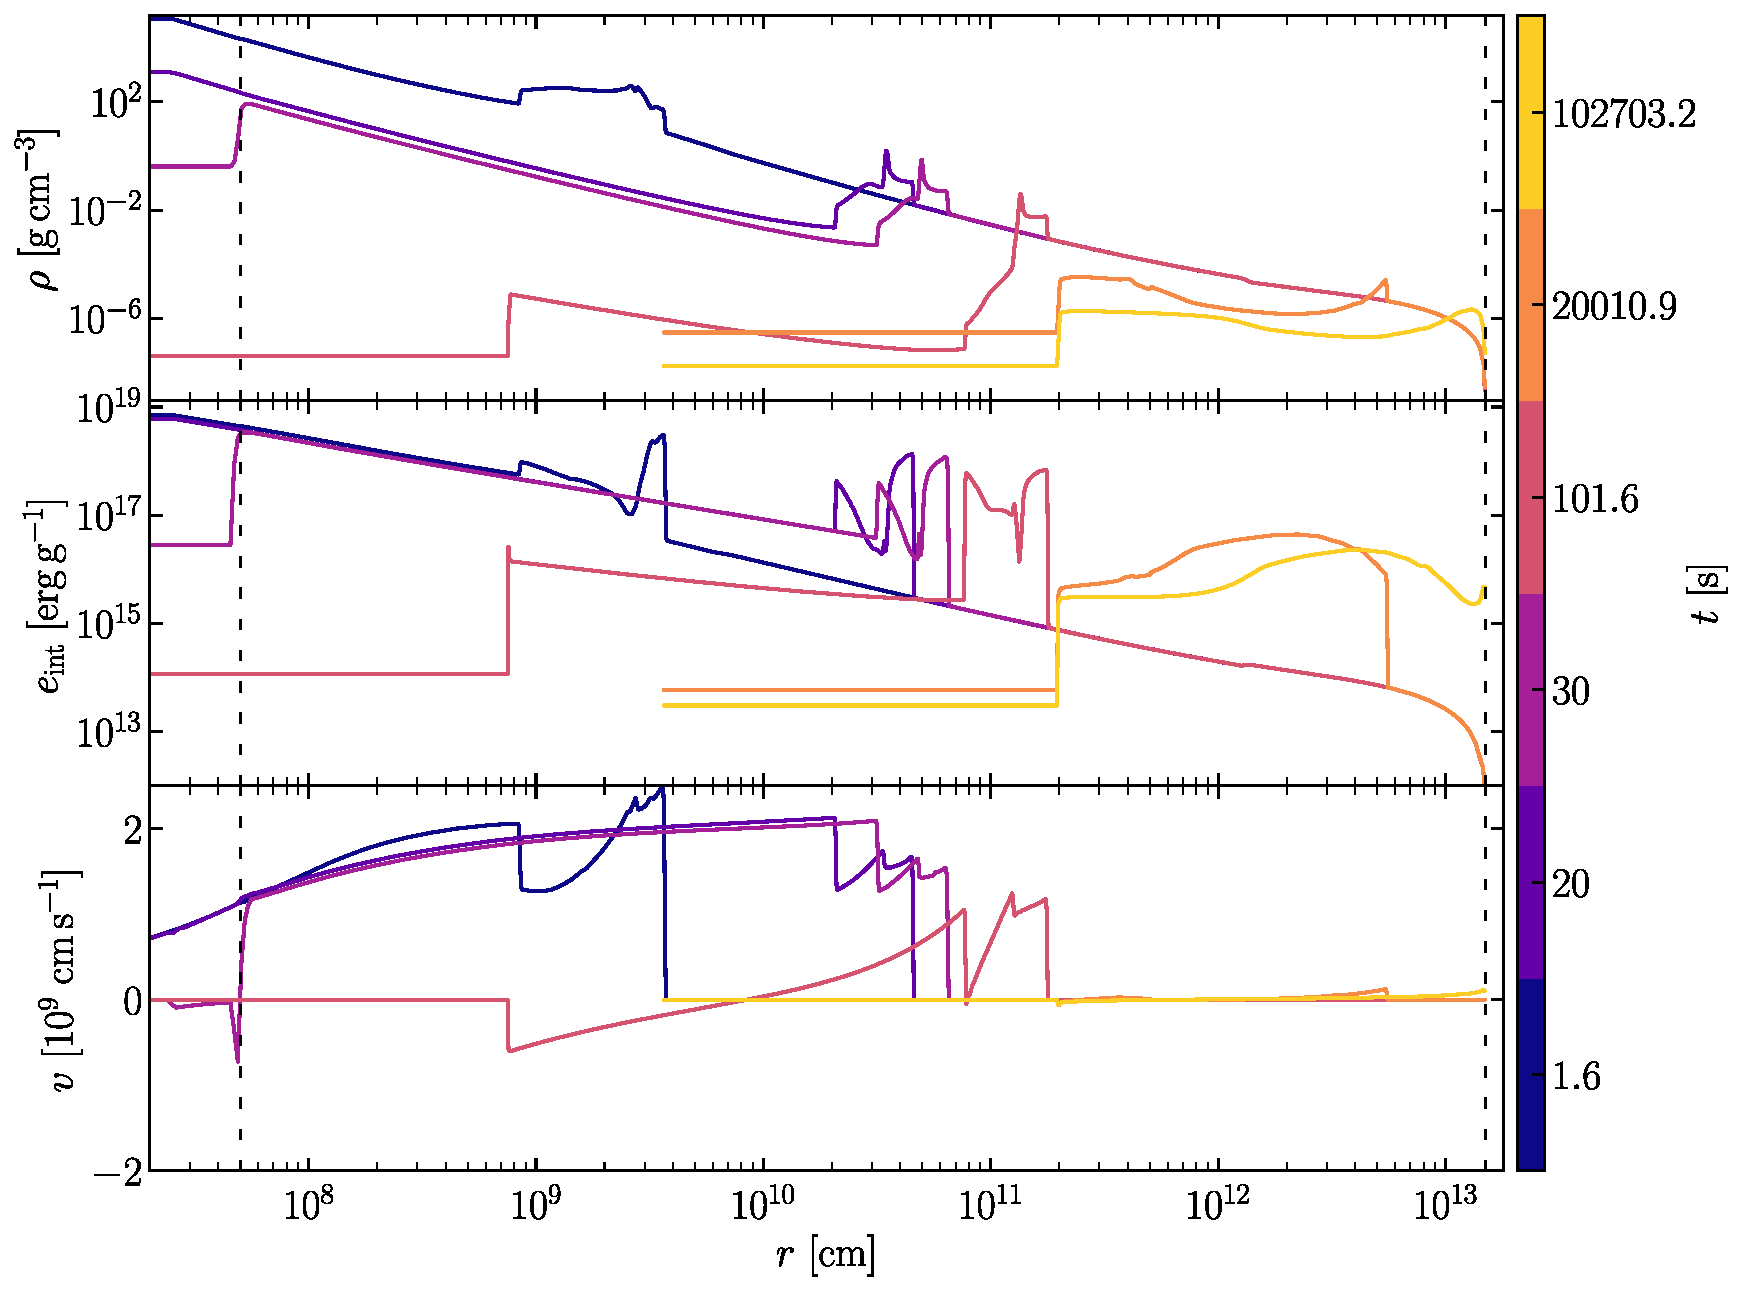
\includegraphics[width=1.0\linewidth]{figures/long_1d.pdf}
    \caption{1D profiles of the density \(\rho\), internal energy \(e_\mathrm{int}\) and velocity \(v\) from time of mapping \(t_\mathrm{map}\) to shock breakout from the stellar surface. The inner boundary for the neutrino wind is located at \(r=500\units{km}\). At \(t = 30\units{s}\), a sharp drop in density and internal energy at the inner boundary indicates the transition to the inflow boundary condition. The boundary of the inflow condition expands at \(100\units{km/s}\) until reaching a maximum radius of \(2 \cdot 10^{11}\units{cm}\) at about \(t=20{,}000\units{s}\). The shock reaches the surface of the star, at \(r=1.5 \cdot 10^{13}\units{cm}\), at a time of about \(100{,}000\units{s}\) post-collapse.}
    \label{fig:long_1d}
\end{figure}

\clearpage

\subsection{Shock propagation \& explosion energy}

In \Cref{fig:long_1d} we can see the velocity of the forward shock drop to very low values as it reaches the stellar surface. This is caused by density gradients in the stellar envelope. According to \cite{Sedov1959}, positive gradients of the \(\rho r^3\) profile will cause a deceleration of the shock wave, whereas negative gradients will accelerate it. This can be seen in \Cref{fig:shock_vel}, where we have plotted the \(\rho r^3\) profile and shock velocity against radius. The shock is originally rapidly accelerated to very high velocities, about \(35{,}000\units{km/s}\), as it escapes the iron core due to the steep, negative density gradient in the Si layer. It is then gradually decelerated after crossing the C+O/He interface to just a few \(100\units{km/s}\) as it reaches the stellar surface. We note that the shock velocity we have obtained is consistent with the 3D simulations of the z9.6 progenitor of \cite{Stockinger2020} as well as the multidimensional simulations of the same progenitor by \cite{Sandoval2021}.

\begin{figure}[ht!]
    \centering
    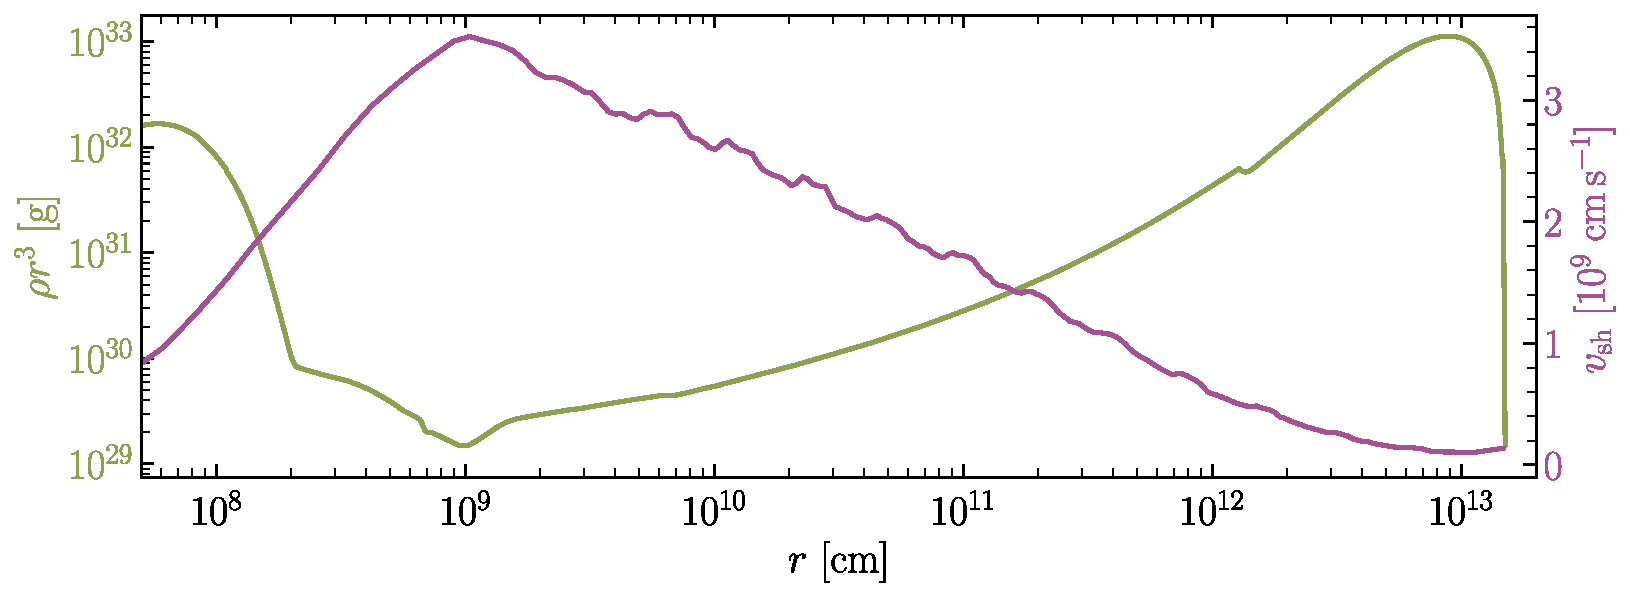
\includegraphics[width=1.0\linewidth]{figures/shock_vel.pdf}
    \caption{Shock velocity (right axis) and \(\rho r^3\) (left axis) radial profiles of z9.6 progenitor.}
    \label{fig:shock_vel}
\end{figure}

Lastly, \Cref{fig:quantities_1d} shows the shock radius, shock velocity and diagnostic explosion energy from \(0.4\units{s}\) to \(30\units{s}\) after collapse. This corresponds to a time slightly after shock revival, until the moment the neutrino wind is shut down and replaced with the inflow boundary condition. We note a smooth continuation of the shock radius and velocity between the data from the initial simulation, in green, and the long term simulation in purple, although the shock velocity is a little noisy. The diagnostic explosion energy shows a slight offset of \(\sim2\%\). This gap is due to different definitions of the diagnostic explosion energy and the need to account for the nuclear EoS before mapping, which is absent after mapping. We can however see an injection of energy of about \(3\%\) from the neutrino wind, resulting in an explosion of \(\sim0.1\units{B}\), where the \emph{Bethe} is defined as \(1\units{B} = 10^{51}\units{erg}\) \citep{Weinberg2006}.

\begin{figure}[ht!]
    \centering
    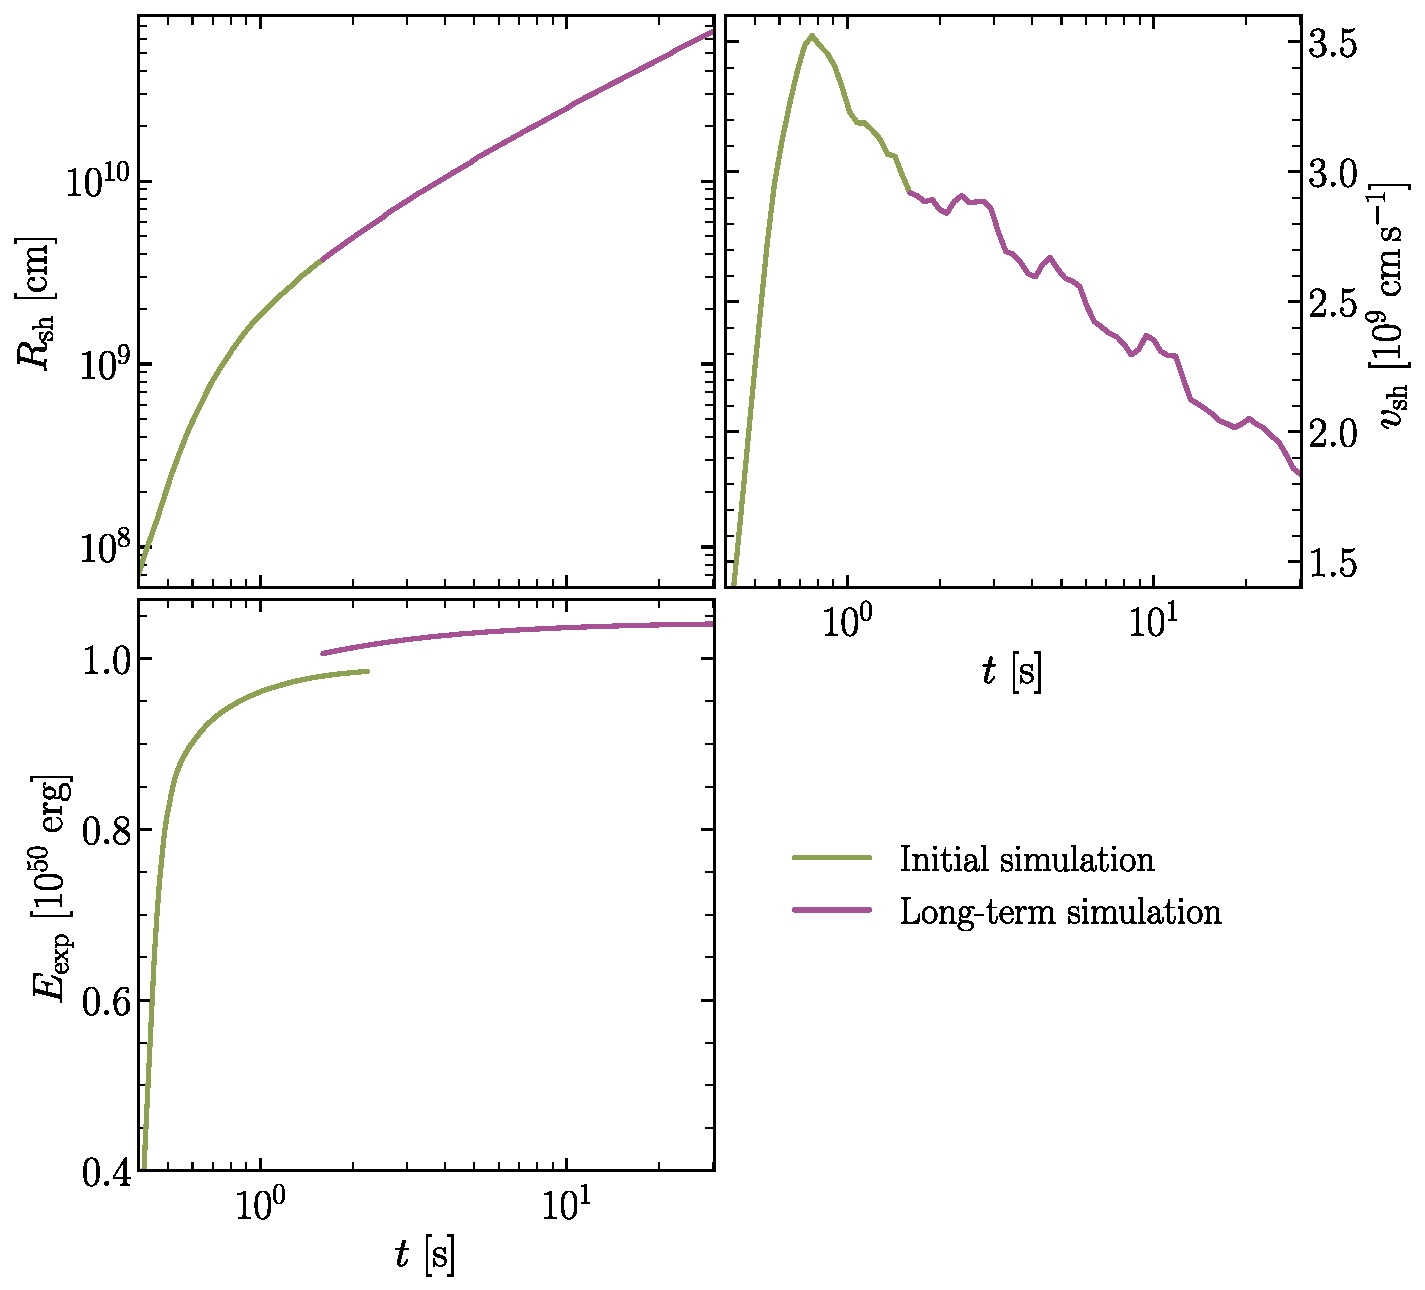
\includegraphics[width=0.9\linewidth]{figures/quantities_1d.pdf}
    \caption{Shock radius (top left), shock velocity (top right), and diagnostic explosion energy (bottom left) from \(0.4\units{s}\) to \(30\units{s}\) after collapse for the z9.6 progenitor. Before mapping, the results are taken from the initial simulation (green line), with a slight overlap with the long-term simulation (purple line) for the diagnostic explosion energy, as data from the initial simulation were available until \(2.2\units{s}\) after collapse.}
    \label{fig:quantities_1d}
\end{figure}

\clearpage

\section{2D simulations} \label{sec:results_2d}

We now look at the 2D simulations of the s12 progenitor. These simulations were run with different neutrino heating factors and wind velocities, as summarised in \Cref{tab:sim_params}.
%In addition, for each of the initial three simulations, with different heating factors, we have run another set of simulations using only the inflow boundary condition instead of the neutrino wind.

\subsection{Wind velocity}

For the 1D simulations, the condition of spherical symmetry forces the formation of a neutrino-driven wind after shock revival, and it is easy to map our neutrino wind condition using the value of the velocity from the profile of the initial simulation. In 2D however, asymmetrical phenomena such as convection and turbulence complicate this picture and can result in regions of accretion and ejection of material around the PNS, which does not map well with our spherically symmetric wind. For this reason, and as was discussed in \Cref{sec:lt_setup}, it was not possible to obtain a realistic wind velocity from the spherically averaged profile of the initial simulation. Consequently, we have decided to run simulations using different wind velocities to explore the impact of this parameter on the long-term evolution of the simulation.

The first two simulations involved the s12 progenitor with a heating factor \(f_\mathrm{heat} = 1.0\). One simulation was ran with a weak wind of \(10{,}000\units{km/s}\), and the other with a strong wind of \(28{,}000\units{km/s}\).

\Cref{fig:s12hf1p0_og} shows slices of the initial s12hf1p0 simulation, showing that at time of mapping \(t_\mathrm{map} = 1.0\units{s}\) the PNS was accreting matter from the north pole and equator, while driving a strong wind at the south pole, with velocities exceeding \(30{,}000\units{km/s}\). As a result, \Cref{fig:s12hf1p0_strong_slice} shows that, after mapping the inner boundary condition, the strong neutrino wind crashes against the still accreting material, launching a shock, as can be seen on the left panel. This shock does not completely extend to the south pole, where the wind was already strong in the initial simulation. The right panel of \Cref{fig:s12hf1p0_strong_slice} shows the continuing accretion of matter on the north pole, while the wind extends at the bottom to a radius of about \(1.2\cdot10^8\units{cm}\), where a termination shock forms around the central region.

\begin{figure}
    \centering
    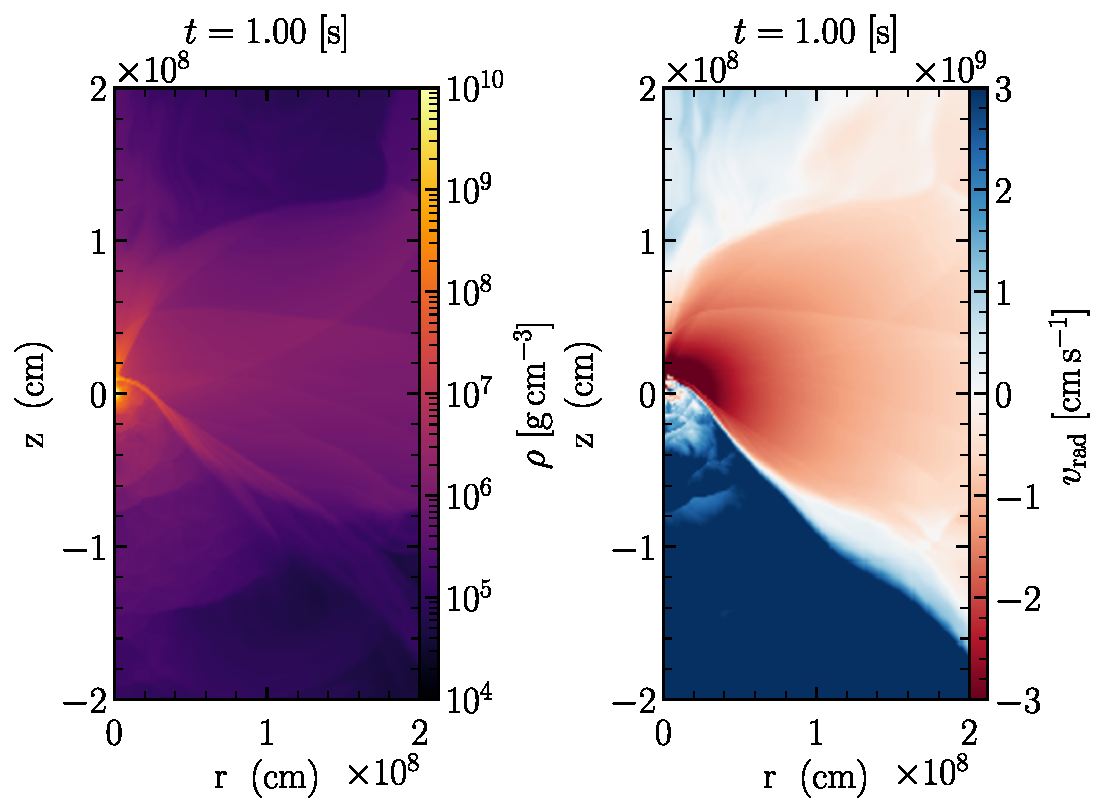
\includegraphics[width=1.0\linewidth]{figures/s12hf1p0_og.pdf}
    \caption{Slices of the initial s12hf1p0 simulation, showing density (left) and radial velocity (right) near the PNS at time of mapping.}
    \label{fig:s12hf1p0_og}
\end{figure}

\begin{figure}[ht!]
    \centering
    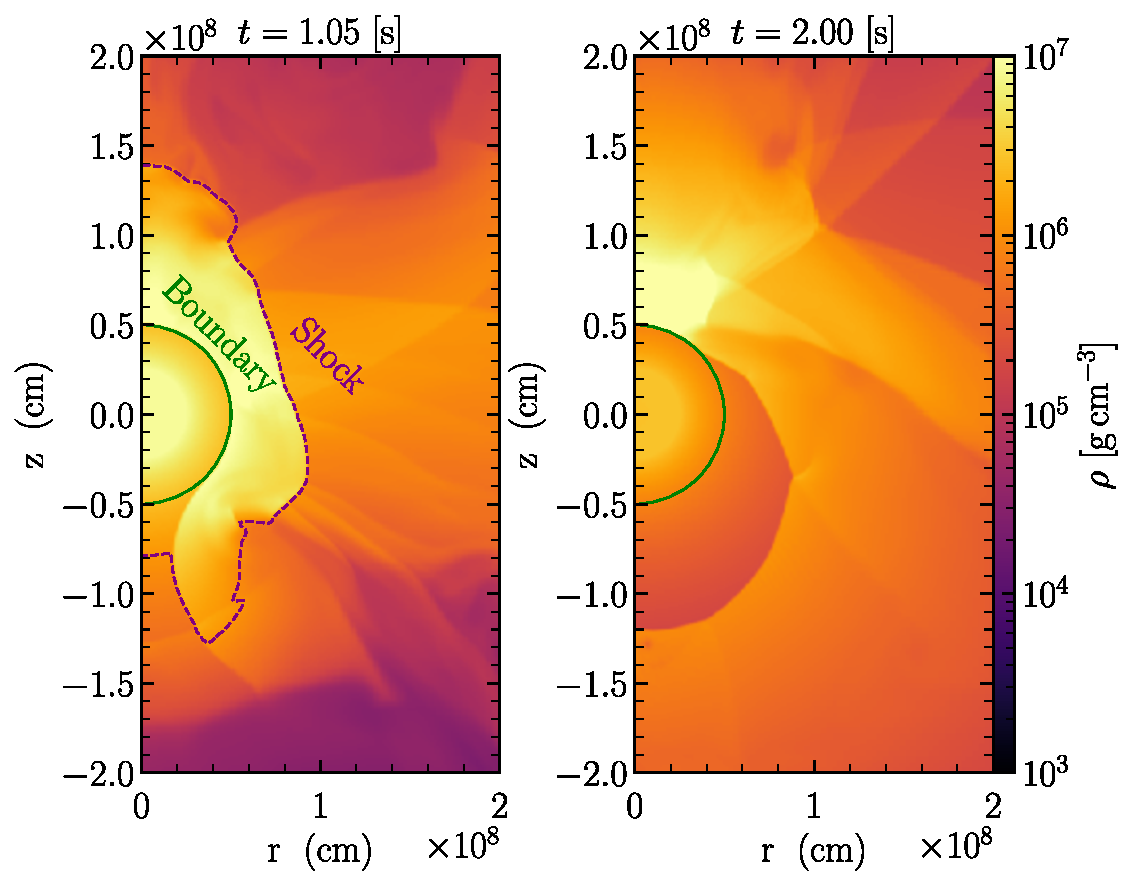
\includegraphics[width=1.0\linewidth]{figures/s12hf1p0_strong_slice_annot.pdf}
    \caption{Slices of the s12hf1p0\_w28e8 simulation, with a strong wind, at \(t=1.05\units{s}\) post-bounce (left) and \(t=2.0\units{s}\) post-bounce (right). A shock is formed (purple contour) by the introduction of the neutrino wind at the inner boundary (green contour).}
    \label{fig:s12hf1p0_strong_slice}
\end{figure}

\clearpage

In addition to the diagnostic explosion energy, it becomes interesting to look at the time evolution of the point mass in the 2D case. Whereas this quantity stayed mostly constant for the 1D simulation, that had no difficulties pushing material out, \Cref{fig:s12hf1p0_strong_quantities} shows a positive gradient of this quantity for the s12hf1p0\_w28e8 simulation, that accretes \(\sim0.1\sunmass\) over the first \(10\units{s}\) of evolution.

\begin{figure}[ht!]
    \centering
    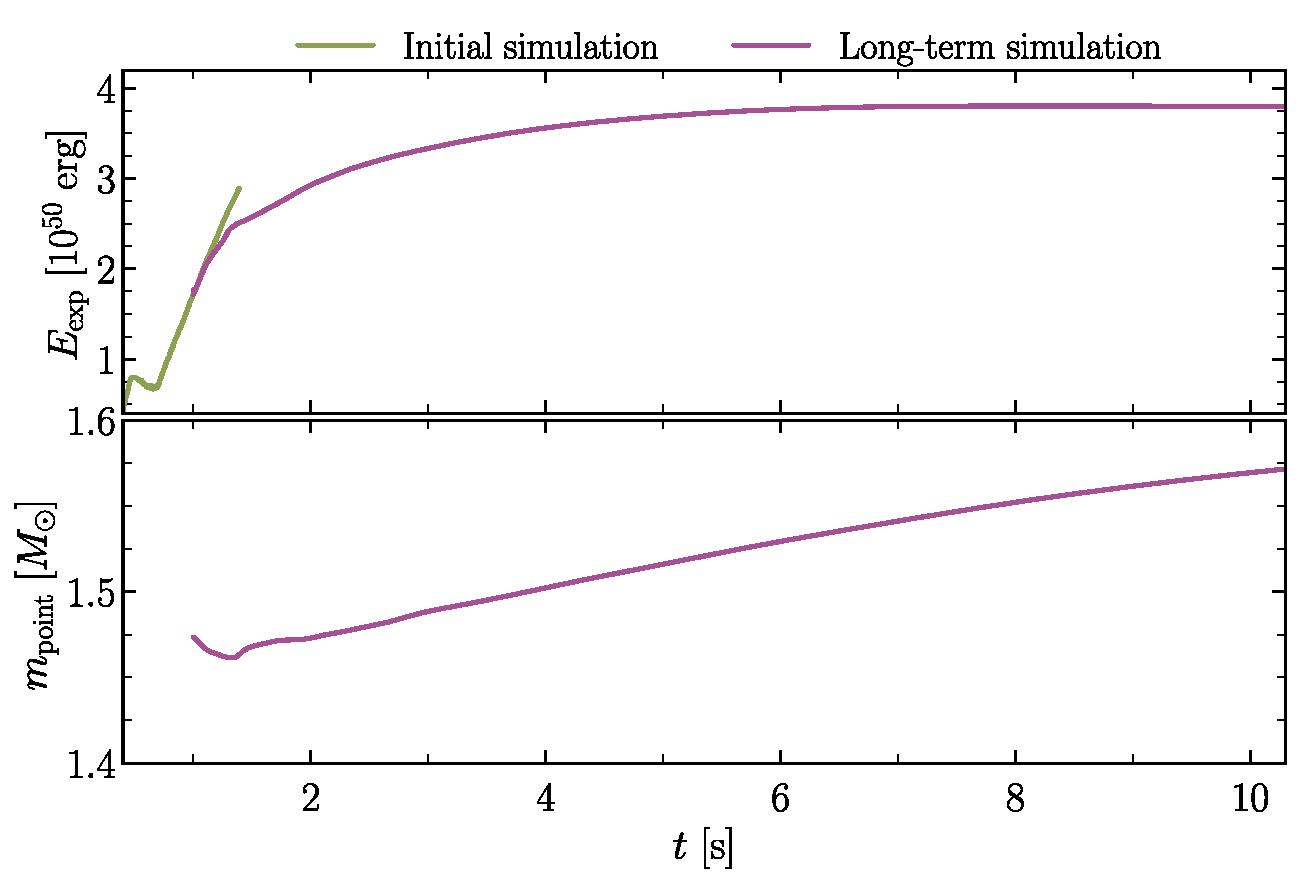
\includegraphics[width=0.9\linewidth]{figures/s12hf1p0_strong_quantities.pdf}
    \caption{Diagnostic explosion energy (top) and point mass (bottom) evolution from time of mapping at \(t_\mathrm{map} = 1.0 \units{s}\) to \(10\units{s}\) post-bounce for the s12hf1p0\_w28e8 simulation.}
    \label{fig:s12hf1p0_strong_quantities}
\end{figure}

We can compare these results with the weak-wind counterpart of this simulation, the s12hf1p0\_w10e8. This simulation uses a wind velocity similar to that of the 1D simulation of the z9.6 progenitor, but is too weak to drive any ejecta in the 2D simulation of the s12 progenitor. \Cref{fig:s12hf1p0_weak_slice} shows a similar view as \Cref{fig:s12hf1p0_strong_slice} for the s12hf1p0\_w10e8 simulation. We see that material keeps accreting on the inner boundary, but the wind is too weak to launch a shock such as for the s12hf1p0\_w28e8 simulation. In the same way, the wind fails to extend to larger radii and material falls back onto the inner region.

\begin{figure}[ht!]
    \centering
    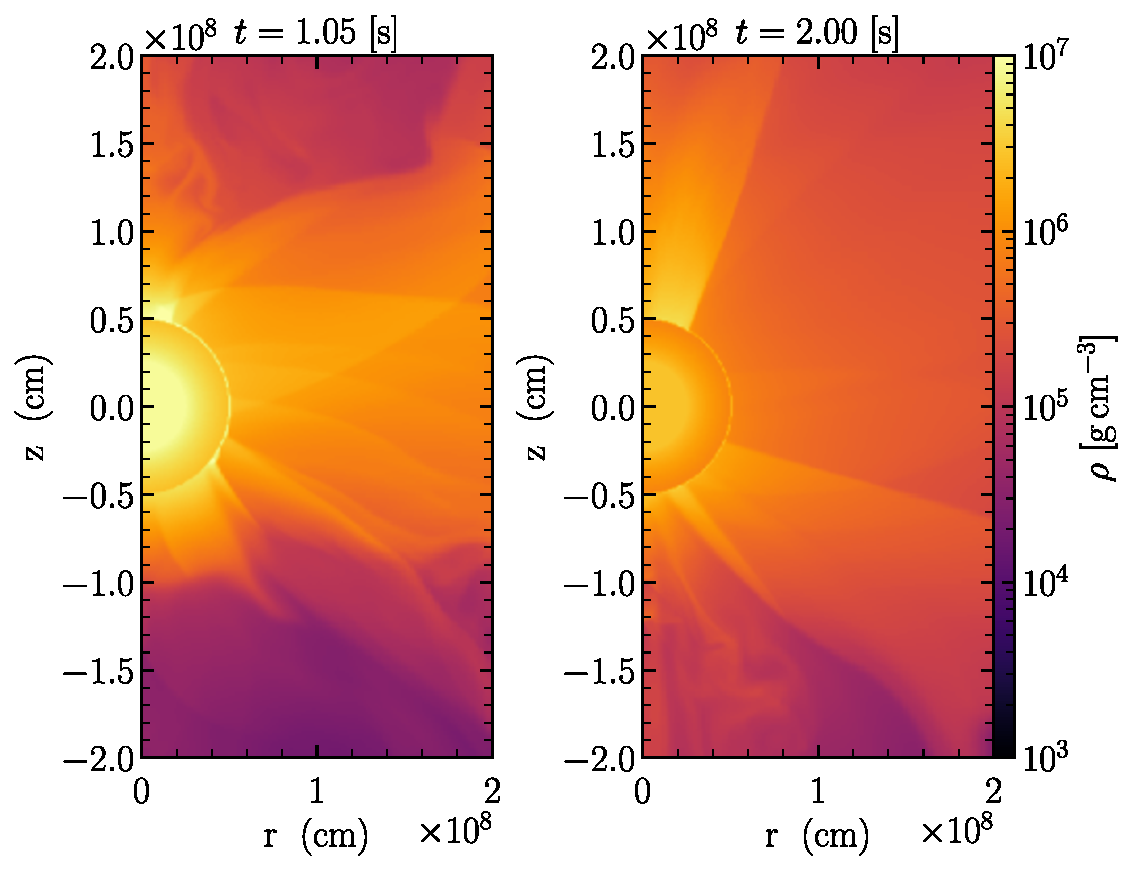
\includegraphics[width=1.0\linewidth]{figures/s12hf1p0_weak_slice.pdf}
    \caption{Slices of the s12hf1p0\_w10e8 simulation, with a weak wind, at \(t=1.05\units{s}\) post-bounce (left) and \(t=2.0\units{s}\) post-bounce (right).}
    \label{fig:s12hf1p0_weak_slice}
\end{figure}

\clearpage

\Cref{fig:s12hf1p0_weak_quantities} shows that the explosion loses \(\sim20\%\) of its energy, whereas \Cref{fig:s12hf1p0_strong_quantities} showed that the strong wind had more than doubled this quantity. On the other hand, the weak wind has accreted twice as much material as the strong wind did, as shown by the evolution of the point mass.

\begin{figure}[ht!]
    \centering
    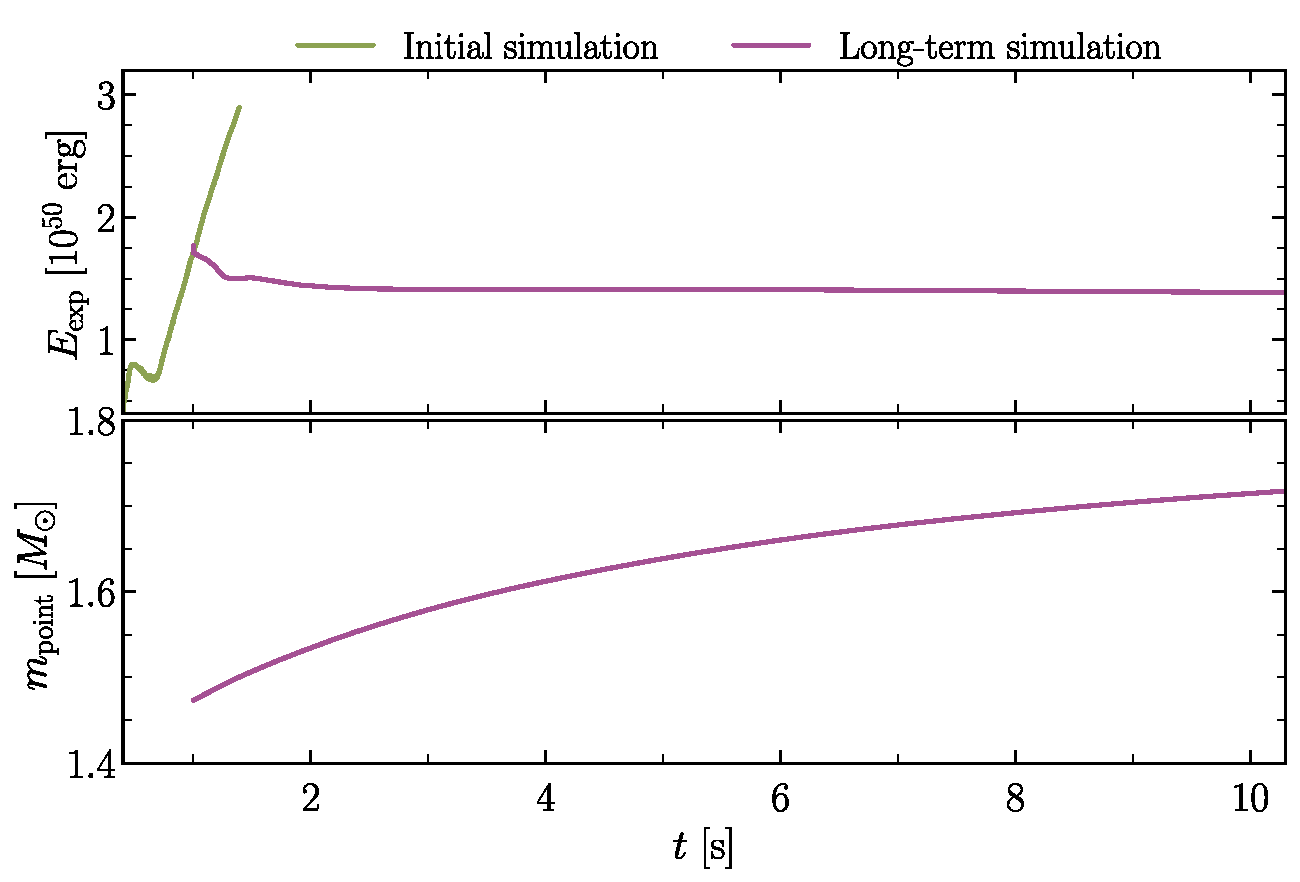
\includegraphics[width=0.9\linewidth]{figures/s12hf1p0_weak_quantities.pdf}
    \caption{Diagnostic explosion energy (top) and point mass (bottom) evolution from time of mapping at \(t_\mathrm{map} = 1.0 \units{s}\) to \(10\units{s}\) post-bounce for the s12hf1p0\_w10e8 simulation.}
    \label{fig:s12hf1p0_weak_quantities}
\end{figure}

We see that the spherical symmetry of our neutrino-driven wind clashes with the asymmetries of the initial simulation, and that if the strong wind better matches the apparent evolution of the explosion energy of the initial simulation, it results in undesirable consequences on the hydrodynamics. However, a higher heating factor can help the formation of a more spherically symmetric ejecta, rendering our neutrino wind possibly more accurate. \Cref{fig:s12hf1p5_og}, showing slices of the initial s12hf1p5 simulation at time of mapping, demonstrate this effect, as the material is more easily driven outward with very few accretion channels onto the PNS due to the slightly larger heating factor.

\begin{figure}
    \centering
    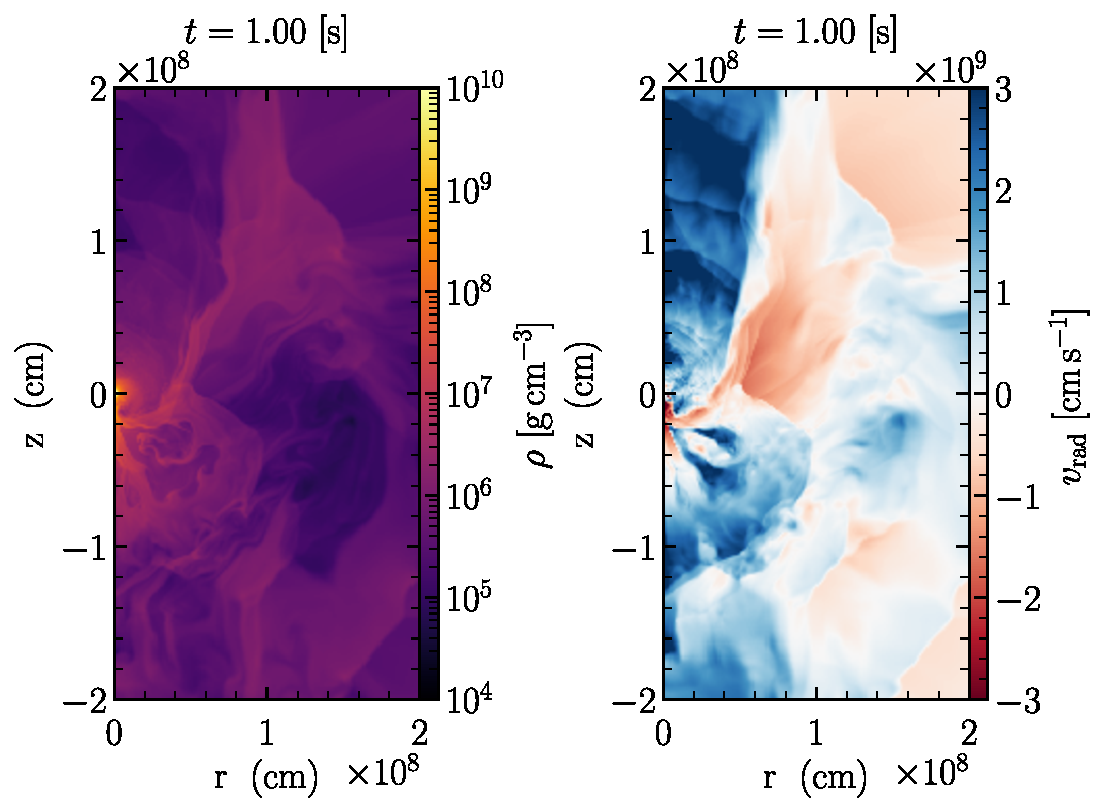
\includegraphics[width=1.0\linewidth]{figures/s12hf1p5_og.pdf}
    \caption{Slices of the initial s12hf1p5 simulation, showing density (left) and radial velocity (right) near the PNS at time of mapping.}
    \label{fig:s12hf1p5_og}
\end{figure}

The wind velocities we used for the two simulations we ran on this progenitor only differ slightly, with the weaker wind being set to \(13{,}000\units{km/s}\) and the stronger wind to \(15{,}000\units{km/s}\). However, as shown in \Cref{fig:s12hf1p5_weak_quantities,fig:s12hf1p5_strong_quantities}, this is enough for the weaker wind to keep the explosion energy mostly constant, whereas the stronger wind succeeds in injecting energy that matches with the initial simulation, without strong hydrodynamical consequences, while almost completely shutting down accretion. We also note that this progenitor initially results in a stronger explosion at moment of mapping compared with the s12hf1p0 simulations.

\begin{figure}
    \centering
    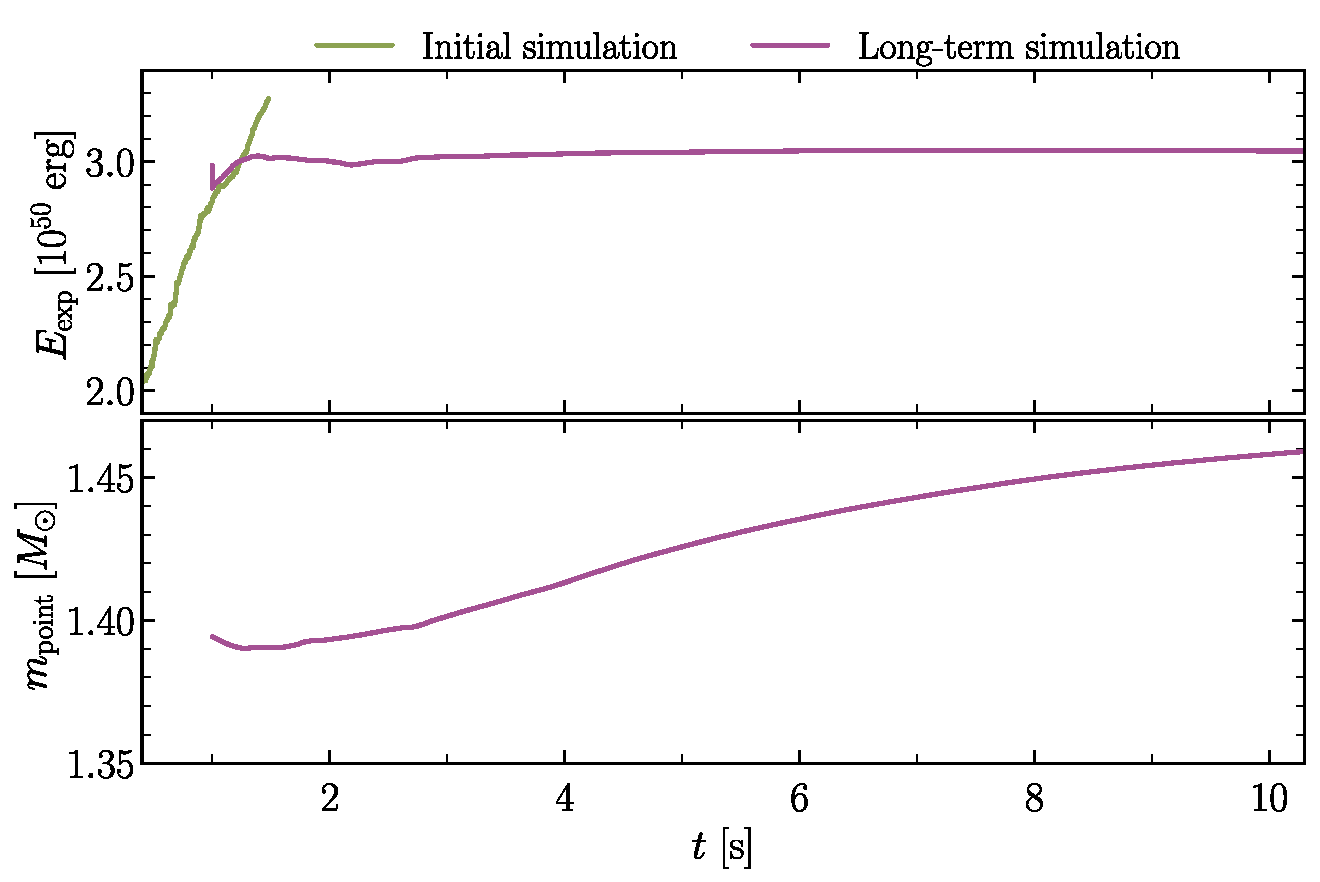
\includegraphics[width=0.9\linewidth]{figures/s12hf1p5_weak_quantities.pdf}
    \caption{Diagnostic explosion energy (top) and point mass (bottom) evolution from time of mapping at \(t_\mathrm{map} = 1.0 \units{s}\) to \(10\units{s}\) post-bounce for the s12hf1p5\_w13e8 simulation.}
    \label{fig:s12hf1p5_weak_quantities}
\end{figure}

\begin{figure}
    \centering
    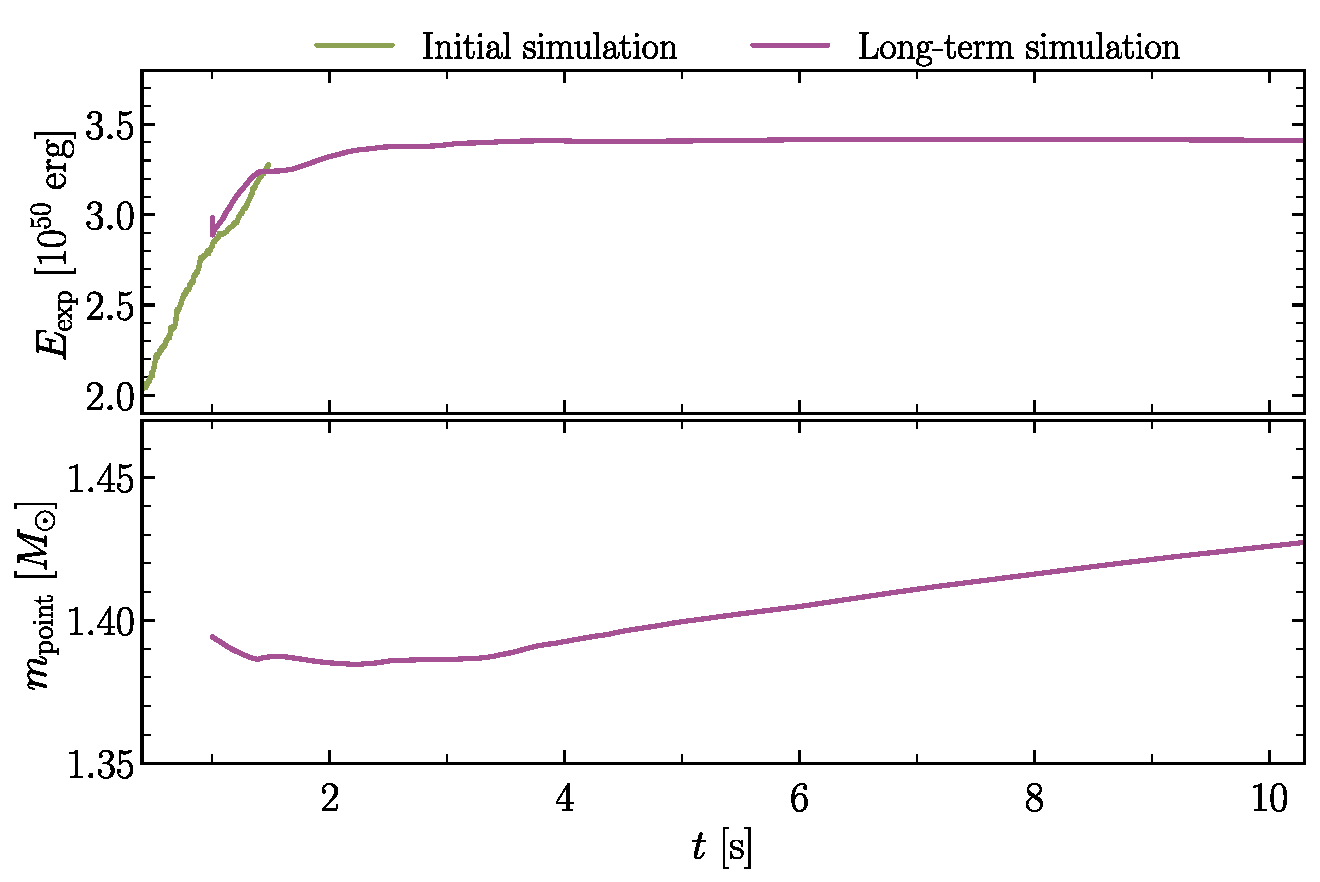
\includegraphics[width=0.9\linewidth]{figures/s12hf1p5_strong_quantities.pdf}
    \caption{Diagnostic explosion energy (top) and point mass (bottom) evolution from time of mapping at \(t_\mathrm{map} = 1.0 \units{s}\) to \(10\units{s}\) post-bounce for the s12hf1p5\_w15e8 simulation.}
    \label{fig:s12hf1p5_strong_quantities}
\end{figure}

\clearpage

We now take a look at the final simulation, that was run with a heating factor \(f_\mathrm{heat} = 2.0\), but only one wind velocity, obtained from the spherically averaged profile of the initial simulation, of \(15{,}600\units{km/s}\). Again, \Cref{fig:s12hf2p0_og} shows the state of the initial simulation at time of mapping, where almost no matter is being accreted, and we can even identify a termination shock at the south hemisphere of the simulation, about \(1.5 \cdot 10^8\units{cm}\) away from the PNS, where a neutrino-driven wind seem to have naturally started to form. Consequently, \Cref{fig:s12hf2p0_slice} shows that there are no noticeable hydrodynamical effects on the simulation due to the mapping of the inner boundary. However, the wind is weaker than in the initial simulation, and the termination shock has fallen back onto the inner boundary at \(2.0\units{s}\) post-bounce, but was enough to keep most of the surrounding material unbound, with one visible accretion channel. This can be observed on \Cref{fig:s12hf2p0_quantities}, that shows that the wind has managed to keep the explosion energy mostly constant after mapping, with only very small accretion, as indicated by the growth of the point mass.

\begin{figure}
    \centering
    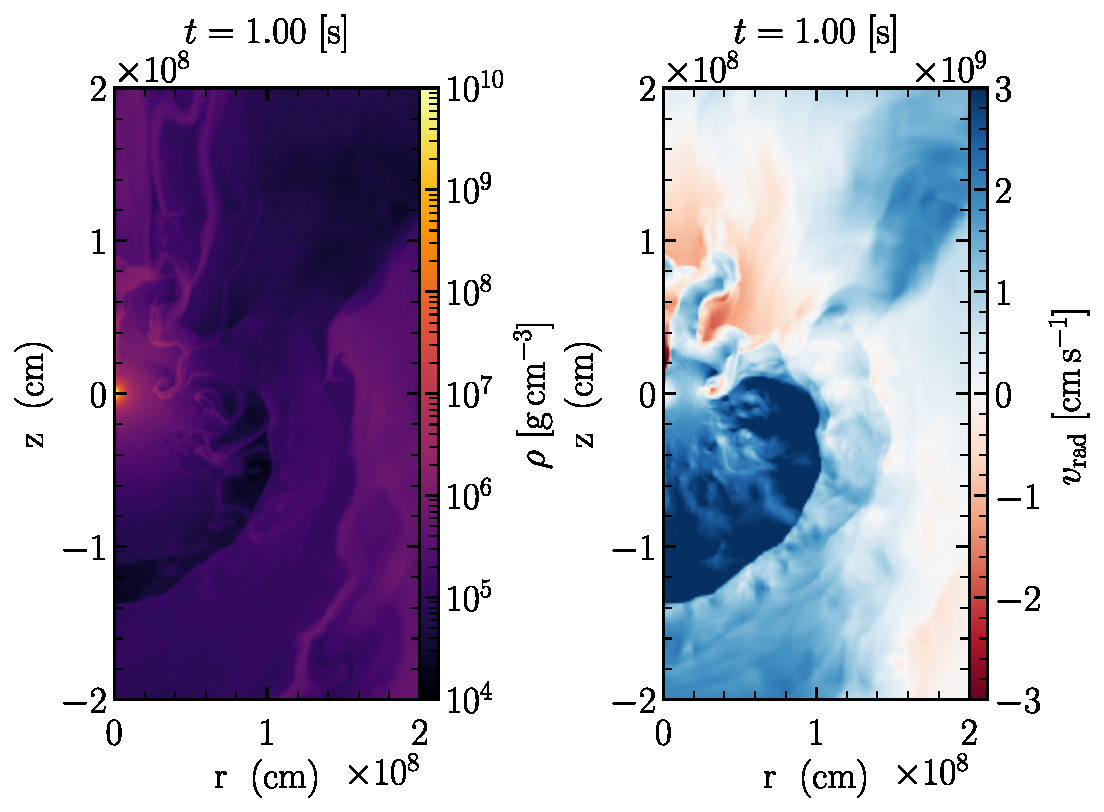
\includegraphics[width=1.0\linewidth]{figures/s12hf2p0_og.pdf}
    \caption{Slices of the initial s12hf2p0 simulation, showing density (left) and radial velocity (right) near the PNS at time of mapping.}
    \label{fig:s12hf2p0_og}
\end{figure}

\begin{figure}
    \centering
    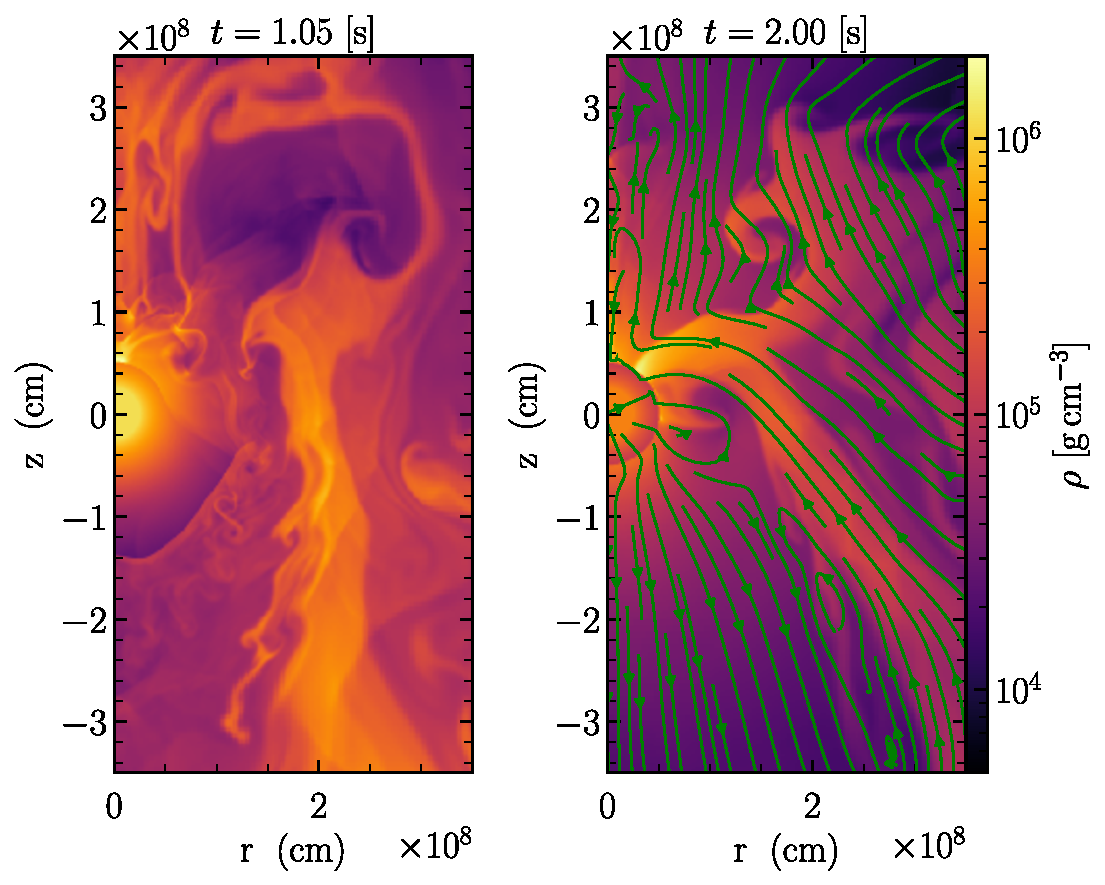
\includegraphics[width=1.0\linewidth]{figures/s12hf2p0_slice.pdf}
    \caption{Slices of the s12hf2p0 simulation at \(t=1.05\units{s}\) post-bounce (left) and \(t=2.0\units{s}\) post-bounce (right). Streamlines of the velocity field are shown in green at \(2.0\units{s}\).}
    \label{fig:s12hf2p0_slice}
\end{figure}

\begin{figure}
    \centering
    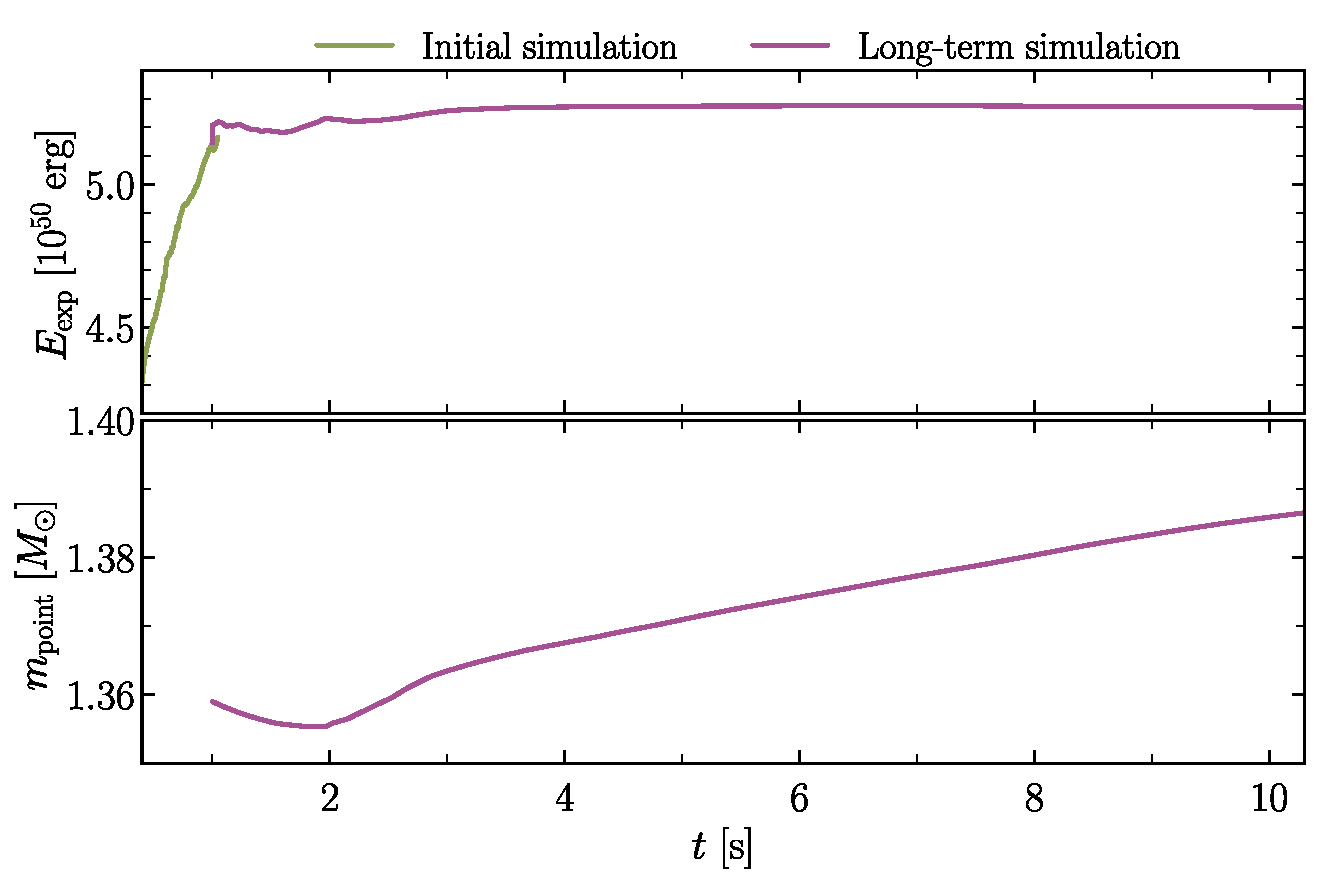
\includegraphics[width=0.9\linewidth]{figures/s12hf2p0_quantities.pdf}
    \caption{Diagnostic explosion energy (top) and point mass (bottom) evolution from time of mapping at \(t_\mathrm{map} = 1.0 \units{s}\) to \(10\units{s}\) post-bounce for the s12hf2p0 simulation.}
    \label{fig:s12hf2p0_quantities}
\end{figure}

\clearpage

\subsection{Shock breakout} \label{sec:breakout}

Finally, \Cref{fig:s12hf1p0_break} shows shock breakout from the stellar surface for the s12hf1p0\_w10e8 and s12hf1p0\_w28e8 simulations. We see that the strong wind has made the forward shock reach the surface at about \(120{,}000\units{s}\), much earlier than for the weak wind, which reaches the surface at around \(210{,}000\units{s}\).

We can in fact obtain an order-of-magnitude estimation of the time of shock breakout. Assuming that the total explosion energy is in the form of kinetic energy, we can express it as a function of the shock velocity \(v_\mathrm{sh}\) and ejecta mass \(M_\mathrm{ej}\):
\begin{equation}
    E_\mathrm{exp} = \frac{1}{2} M_\mathrm{ej} v_\mathrm{sh}^2 \punct{.}
\end{equation}

The ejecta mass being roughly equivalent to the mass of the star at moment of collapse minus the mass of the PNS, we have \(M_\mathrm{ej} \approx 9 \sunmass\) in the case of the s12hf1p0 simulation. Then, solving for the velocity, assuming it is constant, we can estimate the time required for the shock to traverse the entire star, of radius \(R\), corresponding to shock breakout:
\begin{equation}
    t_\mathrm{break} \sim \frac{R}{v_\mathrm{sh}} = \frac{R}{\sqrt{\frac{2 E_\mathrm{exp}}{M_\mathrm{ej}}}} \punct{.}
\end{equation}

Assuming the radius \(R \approx 4 \cdot 10^{13}\units{cm}\) and ejecta mass \(M_\mathrm{ej} \approx 9 \sunmass\) to be the same in both the s12hf1p0\_w10e8 and s12hf1p0\_w28e8 simulations, we can compare this quantity for the two simulations using the explosion energies shown in \Cref{fig:s12hf1p0_weak_quantities,fig:s12hf1p0_strong_quantities} to find
\begin{gather}
    t_\mathrm{break,weak} = \frac{R}{\sqrt{\frac{2E_\mathrm{exp,weak}}{M_\mathrm{ej}}}} \approx 320{,}000\units{s} \punct{,} \\
    t_\mathrm{break,strong} = \frac{R}{\sqrt{\frac{2E_\mathrm{exp,strong}}{M_\mathrm{ej}}}} \approx 196{,}000\units{s} \punct{,}
\end{gather}

where \(t_\mathrm{break,weak}\) and \(E_\mathrm{exp,weak} = 1.35 \cdot 10^{50}\units{erg}\) are the breakout time and explosion energy for the s12hf1p0\_w10e8 simulation, and \(t_\mathrm{break,strong}\) and \(E_\mathrm{exp,strong} = 3.75 \cdot 10^{50}\units{erg}\) are the breakout time and explosion energy for the s12hf1p0\_w28e8 simulation. This quantities compare with the results of the simulations, shown in \Cref{fig:s12hf1p0_break}, within a factor of 2. Furthermore, taking the ratio of these quantities gives
\begin{equation}
    \frac{t_\mathrm{break,weak}}{t_\mathrm{break,strong}} = \sqrt{\frac{E_\mathrm{exp,strong}}{E_\mathrm{exp,weak}}} \approx 1.66 \punct{.}
\end{equation}

This tells us that shock breakout must happen \(\sim1.66\) times faster with the strong wind than with the weak wind, which compares quite well with \Cref{fig:s12hf1p0_break}.

\begin{figure}[ht!]
    \centering
    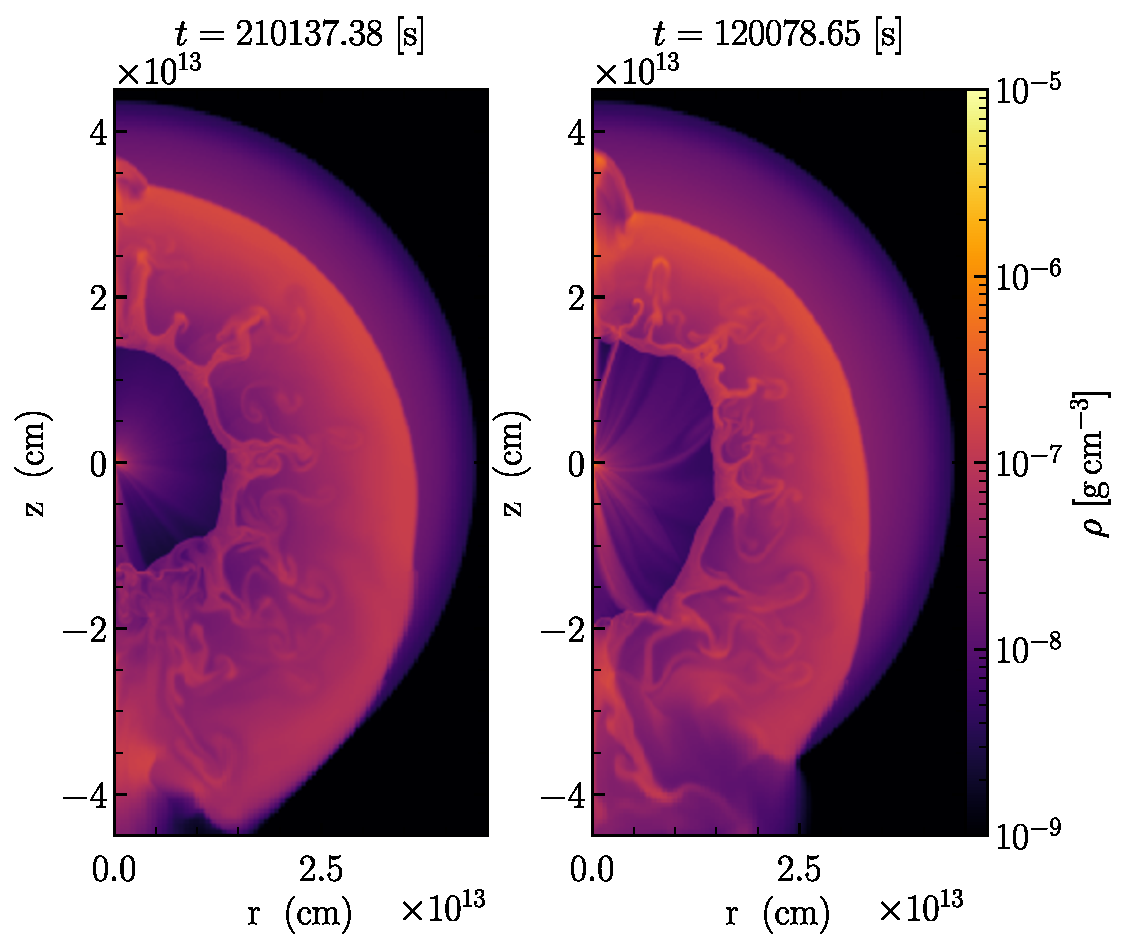
\includegraphics[width=1.0\linewidth]{figures/s12hf1p0_break.pdf}
    \caption{Density plots of the s12hf1p0\_w10e8 (left) and s12hf1p0\_w28e8 simulations (right), showing shock breakout from the stellar surface.}
    \label{fig:s12hf1p0_break}
\end{figure}
